
\section{Transistor}
\vspace{-0.2cm}
\subsection{Bipolarer Transistor}
\vspace{-0.2cm}
\subsubsection{Wirkungsprinzip}
Ein Bipolartransistor besteh aus drei dünnen dotierten Halbleiterschichten, d.h. aus zwei pn-Übergängen. Gemäss der Reihenfolge und dem Dotierungstyp der Schichtung werden Bipolartransistoren in npn- und pnp-Typen unterteilt.\newline Als Leistungstransistoren werden überwiegend npn- Transistoren in der Emmitter-Schaltung verwendet\newline
\hspace*{2cm}
\begin{tabular}{ccc}
     \textbf{Wirkungsprinzip}&\textbf{Aufbau}&\textbf{Schaltzeichen}\\
     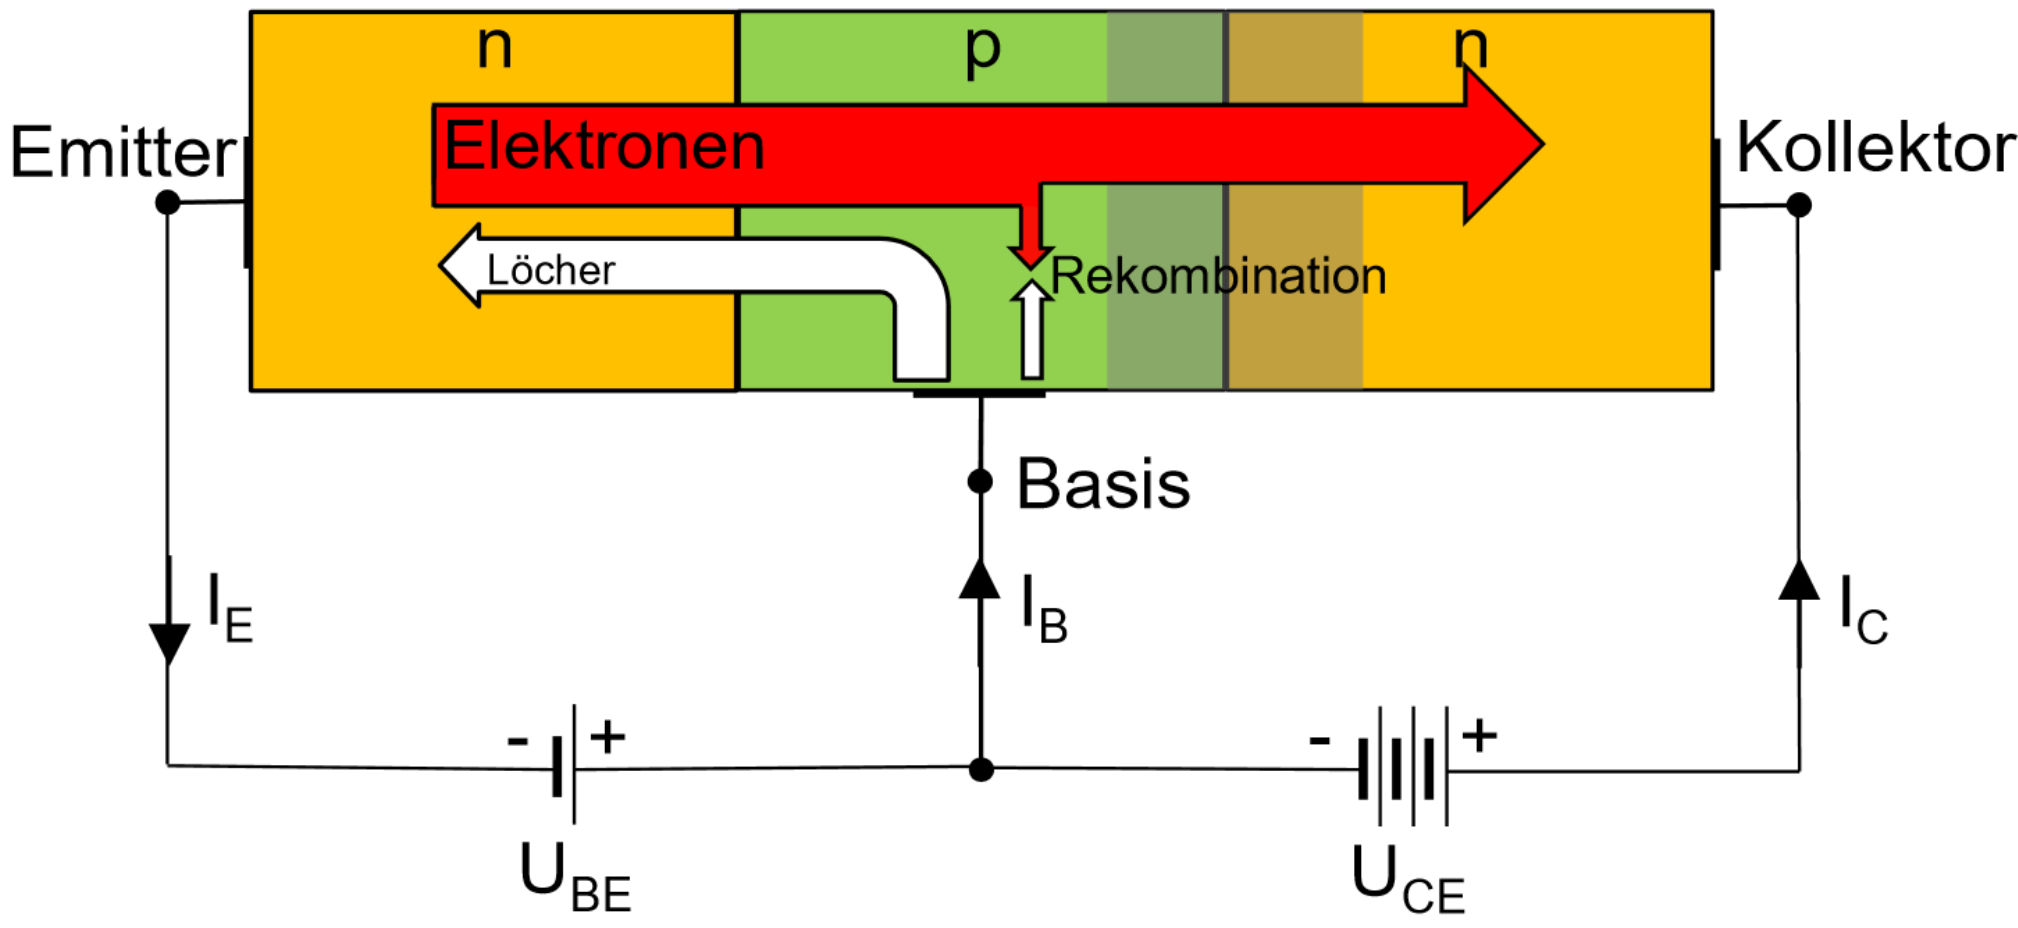
\includegraphics[width=0.35\linewidth]{images/npnTransistor}&
     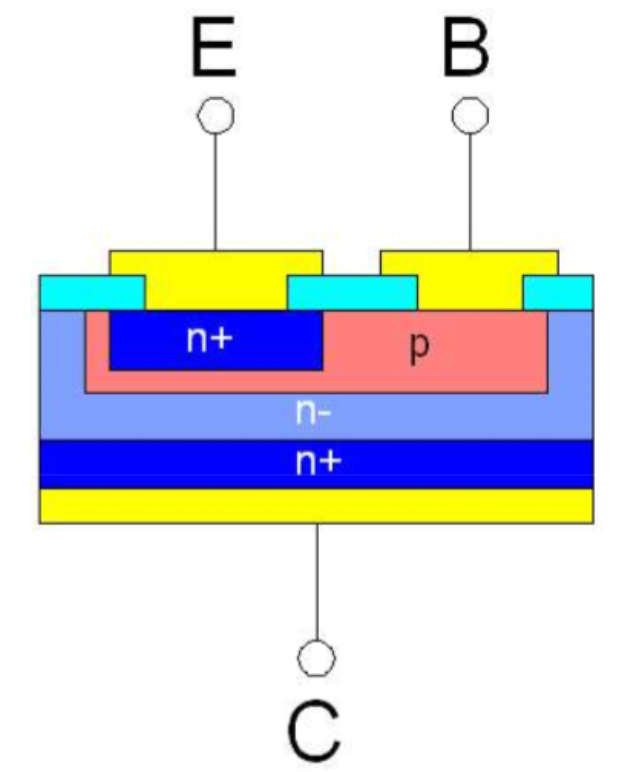
\includegraphics[width=0.15\linewidth]{images/aufbautransnpn}&
     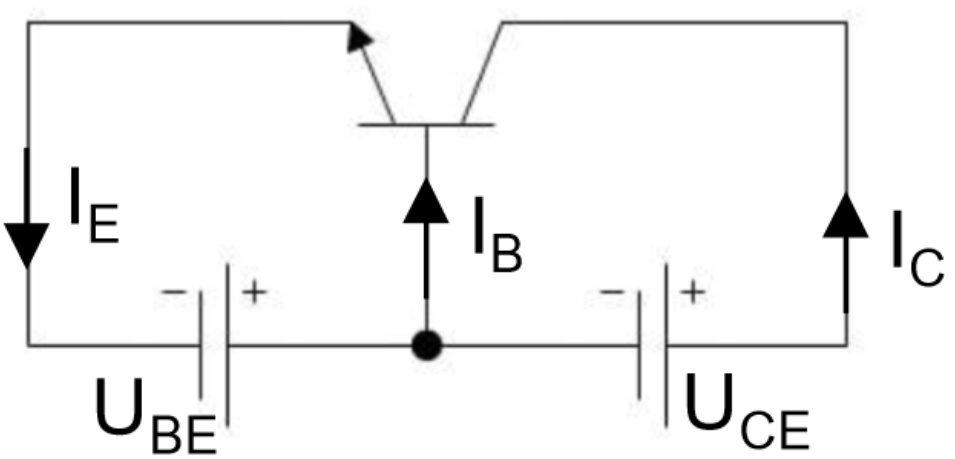
\includegraphics[width=0.25\linewidth]{images/esbtransnpn} \\
\end{tabular}

\subsubsection{Schaltverhalten}
\begin{minipage}{0.6\linewidth}
    \begin{wrapfigure}{r}{4cm}
        \includegraphics[width=\linewidth]{images/npnTransemitter}
    \end{wrapfigure}
    \raggedright
    \textbf{Im Sättigungsbreich} ist der Basisstrom so gross, dass sich in der Basiszone mehr Ladungsträger befinden als für den Kollektorstrom nötig ist.\newline\newline
    Die beiden pn-Übergänge sind in die Durchlassrichtung polarisiert.\newline
    $ U_{BE}>U_{CE} $ und $ U_{BC}>0 $\newline\newline
    Im Verstärkungsbereich gilt: $ \beta = \dfrac{I_C}{I_B} $\newline \newline
    \textbf{Im Schaltbetrieb} werden die Arbeitspunkte \textbf{I} (vorwärts sperrend) und \textbf{III} (Durchlassbetrieb -Sättigung) verwendet.
\end{minipage}
\begin{minipage}{0.4\linewidth}
    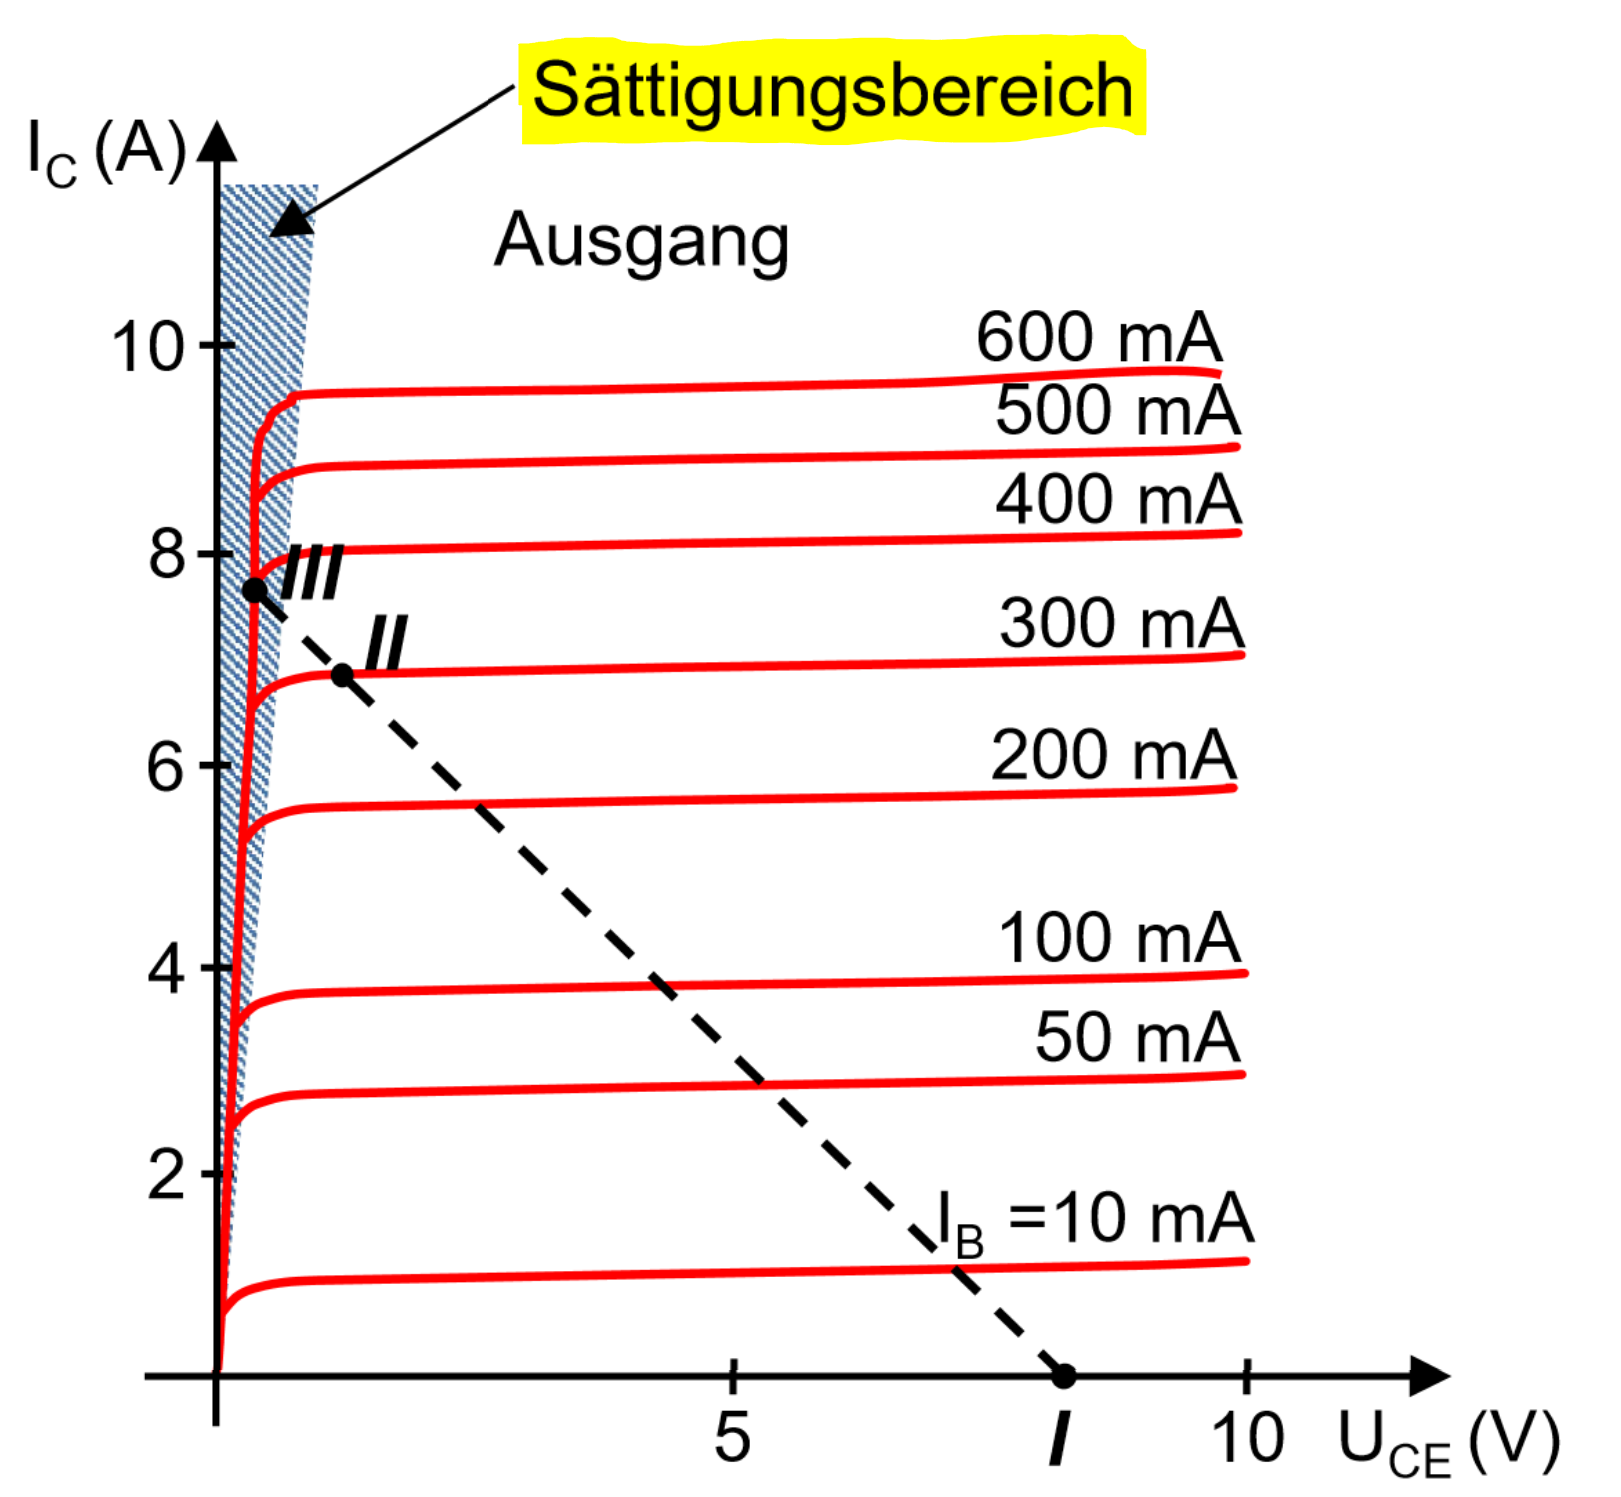
\includegraphics[width=0.8\linewidth]{images/npnTranskennlinie}
\end{minipage}
\subsubsection{Kennwerte}%TODO Leftaligned
\begin{tabularx}{0.5\linewidth}{l p{7cm}} 
    \textbf{$ U_{CES} $}&\textbf{Kollektor-Emitter-Sperrspannung}\\
    &Der höchstzulässige Wert der $ U_{CES} $bei Ansteuerung mit einer negativen $ U_{BE} $\\
    \textbf{$ U_{CE0} $}&\textbf{Kollektor-Emitter-Sperrspannung}\\%RICHTIG??
    &Der höchstzulässige Wert der $ U_{CE} $ bei offenem Basisanschluss\\
    \textbf{$ I_{CAVM} $}&\textbf{Kollektor-Dauergrenzstrom}\\
    &Der höchstzulässige Wert des Gleichstrom-Mittelwerts bei vorgegebener Temperatur\\
    \textbf{$ I_{CRM} $}&\textbf{periodischer Kollektor-Spitzenstrom}\\
    &der höchstzulässige Wert eines Pulsstromes mit angegebener Periodendauer und Einschaltdauer\\
\end{tabularx}
\begin{minipage}{0.5\linewidth}
    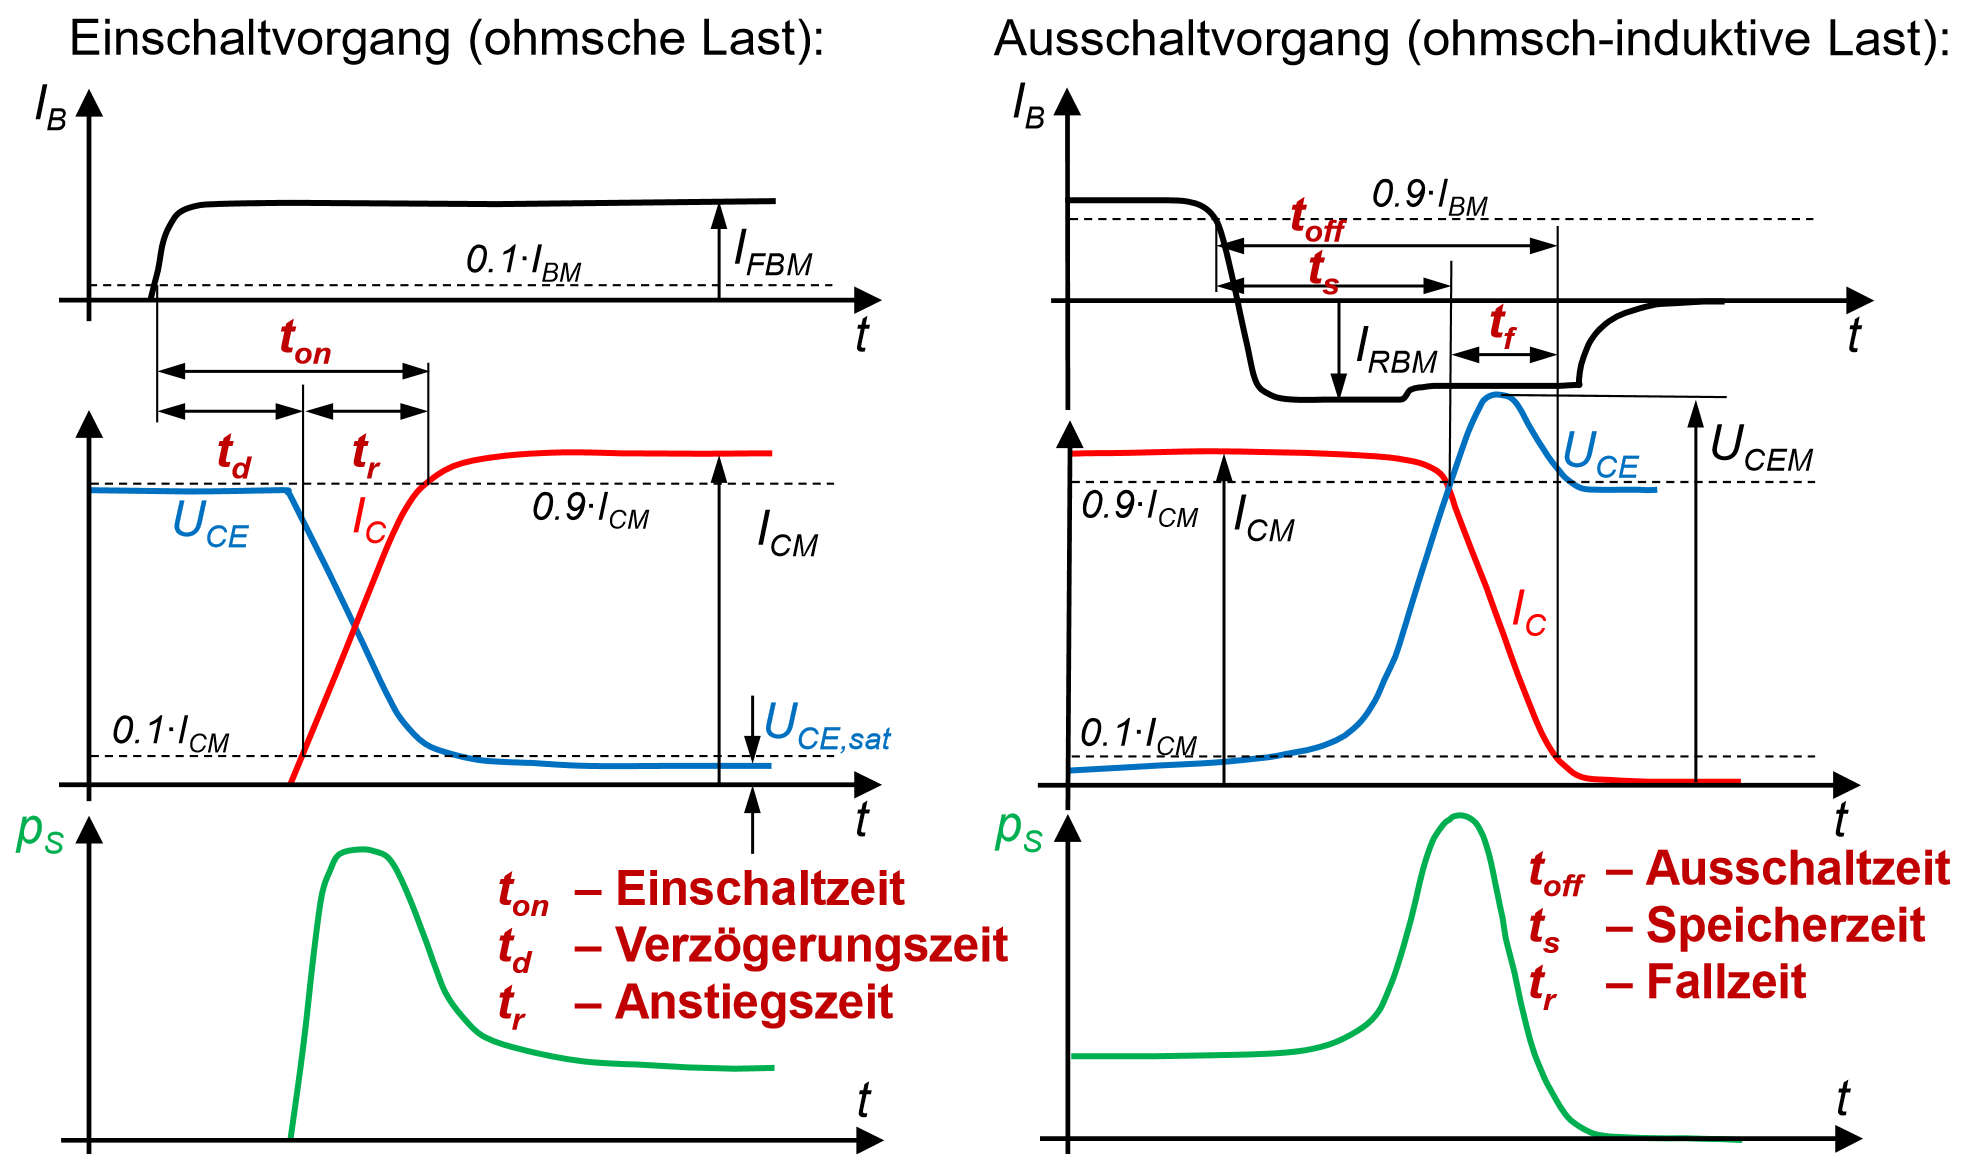
\includegraphics[width=\linewidth]{images/npnTransESV}
\end{minipage}

\begin{minipage}{0.5\linewidth}
    \subsubsection{Verluste}
    \begin{itemize}
        \item Einschaltverluste
        \item Ausschaltverluste
        \item Durchlassverluste
        \item Sperrverluste
    \end{itemize}
\end{minipage}
\begin{minipage}{0.5\linewidth}
    \hspace{0.5cm}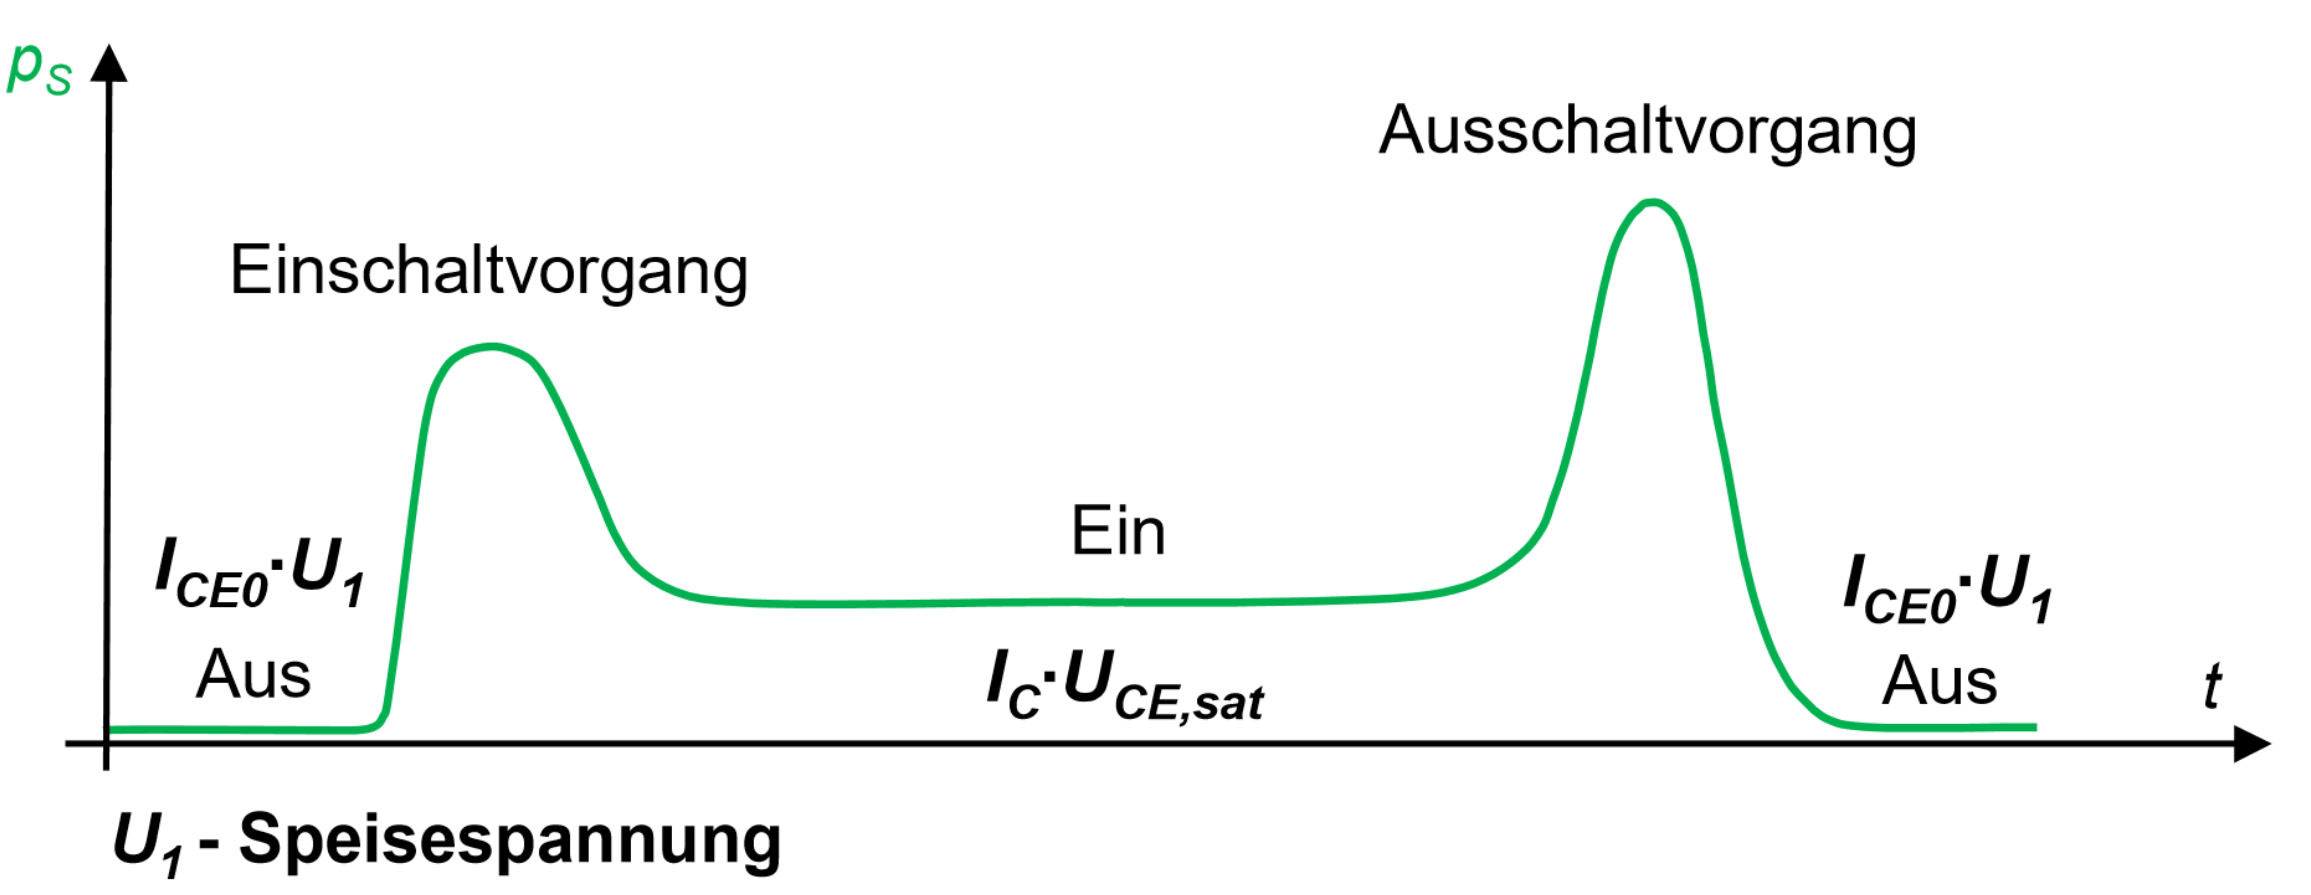
\includegraphics[width=\linewidth]{images/npnTransVerluste}
\end{minipage}
\clearpage

\vspace*{-1cm}
\subsection{Darlington-Transistoren}
\begin{wrapfigure}{r}{2cm}
    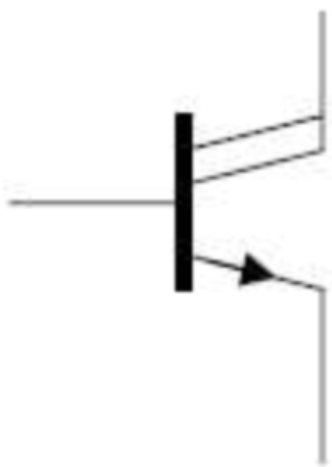
\includegraphics[width=\linewidth]{images/darlingtonSymbol}
\end{wrapfigure}
Der Stromverstärkungsfaktor der Leistungstransistoren ist relativ klein. Deswegen ist ein straker Basisstrom für diese Transistoren notwendig. Ein Darlington-Transistor löst diese Problem.

\begin{minipage}{0.6\linewidth}
    \subsubsection{Formeln}
    \vspace{-0.2cm}
    $ \beta = \text{Kleinsignaglversätrkung}$\newline
    $B = \text{Grosssignalverstärkung}$
    \vspace{-0.2cm}
    \[ \beta_1 = \dfrac{i_{C1}}{i_{B1}} \qquad \beta_2 = \dfrac{i_{C2}}{i_{B2}} \]    
    \[ i_{E1} = i_{C1}+i_{B1}=(1+\beta_1)i_{B1} = i_{B2} \]
    \[ i_{C2} = \beta_2 i_{B2} = \beta_2 i_{E1} = \beta_2 (1 + \beta_1)i_{B1}=\beta_{ges}i_{B1} \]
    \[ \beta_{ges} = \beta_2(1 + \beta_1) \approx \beta_1 \beta_2 \]    
\end{minipage}
\begin{minipage}{0.3\linewidth}
    \subsubsection{Aufbau}
    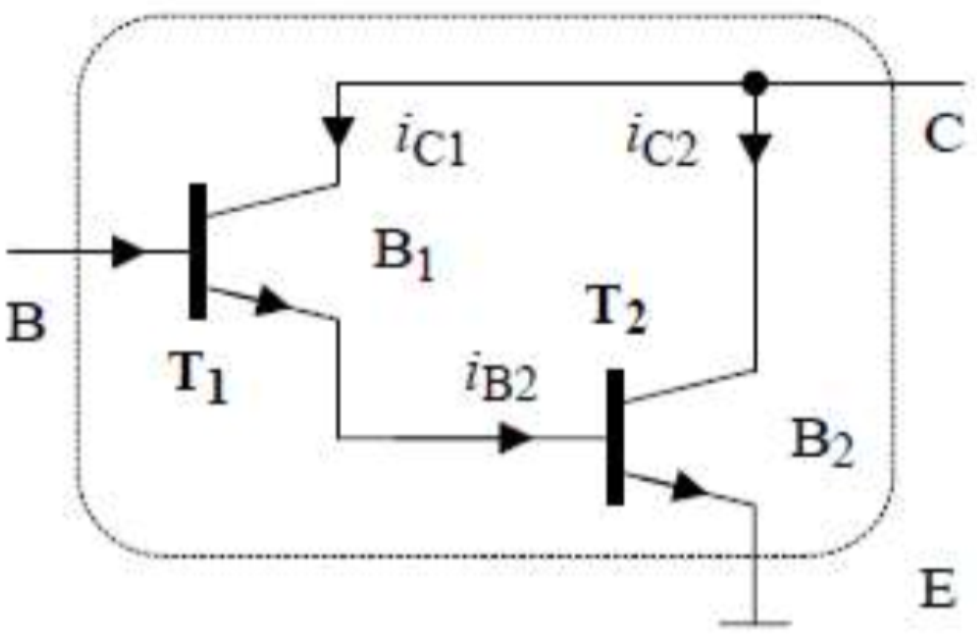
\includegraphics[width=\linewidth]{images/darlingtonaufbau}
\end{minipage}
 \vspace{-0.2cm}
\subsubsection{Vor und Nachteile}
\vspace{-0.5cm}
\begin{multicols}{2}
    \begin{minipage}{\linewidth}
        \begin{itemize}
            \item [+] Gleichbleibender Platzbedarf, höhere Stromverstärkung
            \item [+] $ B \approx B_1 \cdot B_2 $ im Bereich <1000 
            \item [+] $ \beta \approx \beta_1 \cdot \beta_2 $ im Bereich <50'000
        \end{itemize}
    \end{minipage}
    
    \begin{minipage}{1.2\linewidth}
        \begin{itemize}
            \item [-] grosse Phasenverschiebung
            \item [-] für Hochfrequenzanwendungen ungeeingnet
            \item [-] langsame Schaltzeiten
            \item [-] doppelte Basis-Emitter-Spannung
        \end{itemize}
    \end{minipage}
\end{multicols}
Für effiziente Schaltanwendungen eignen sich Darlingtontransistoren wegen diesen Nachteilen kaum.
 \vspace{-0.2cm}
\subsection{MOSFET}
\begin{wrapfigure}{r}{7cm}
    \vspace{-1cm}
    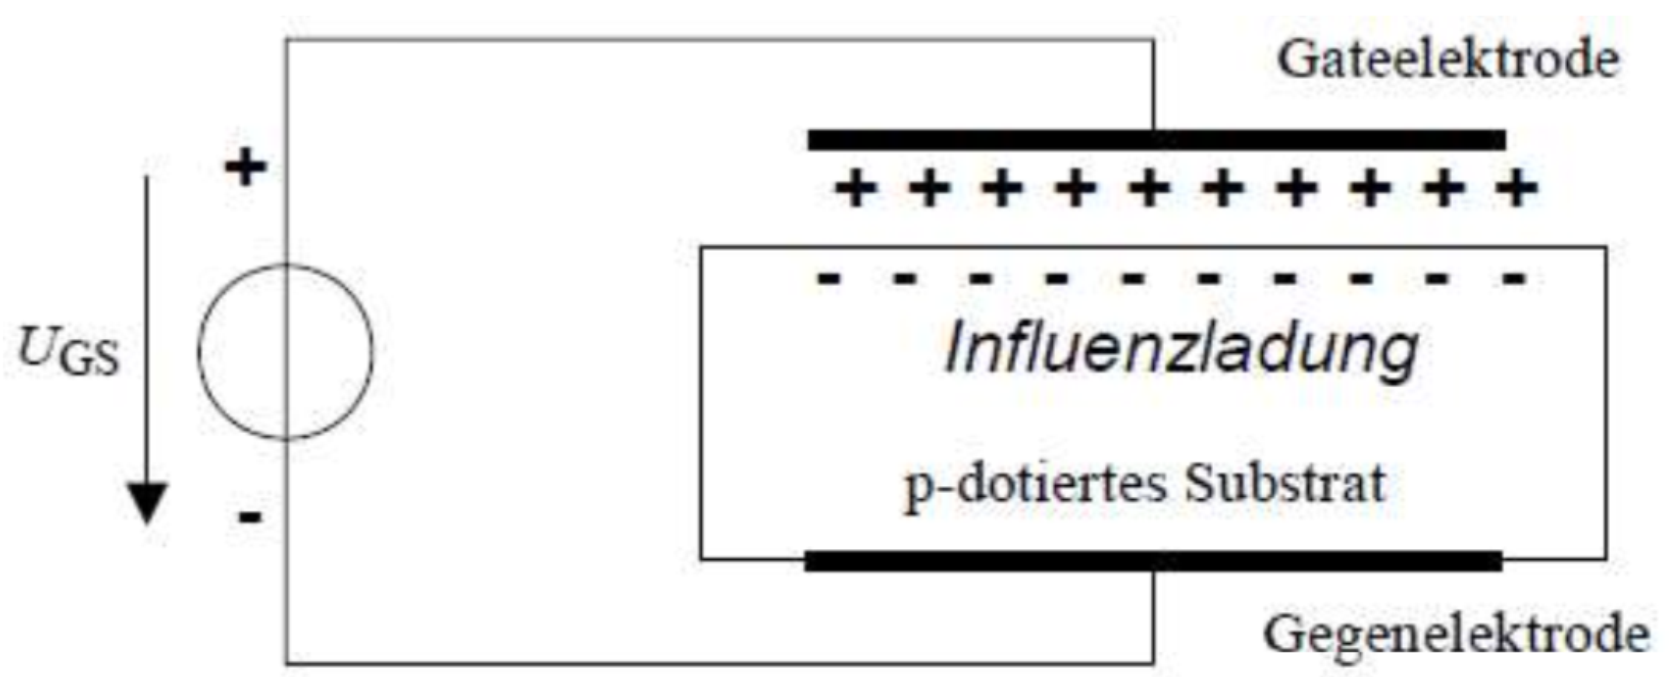
\includegraphics[width=\linewidth]{images/mosfetprinz}
    \newline
    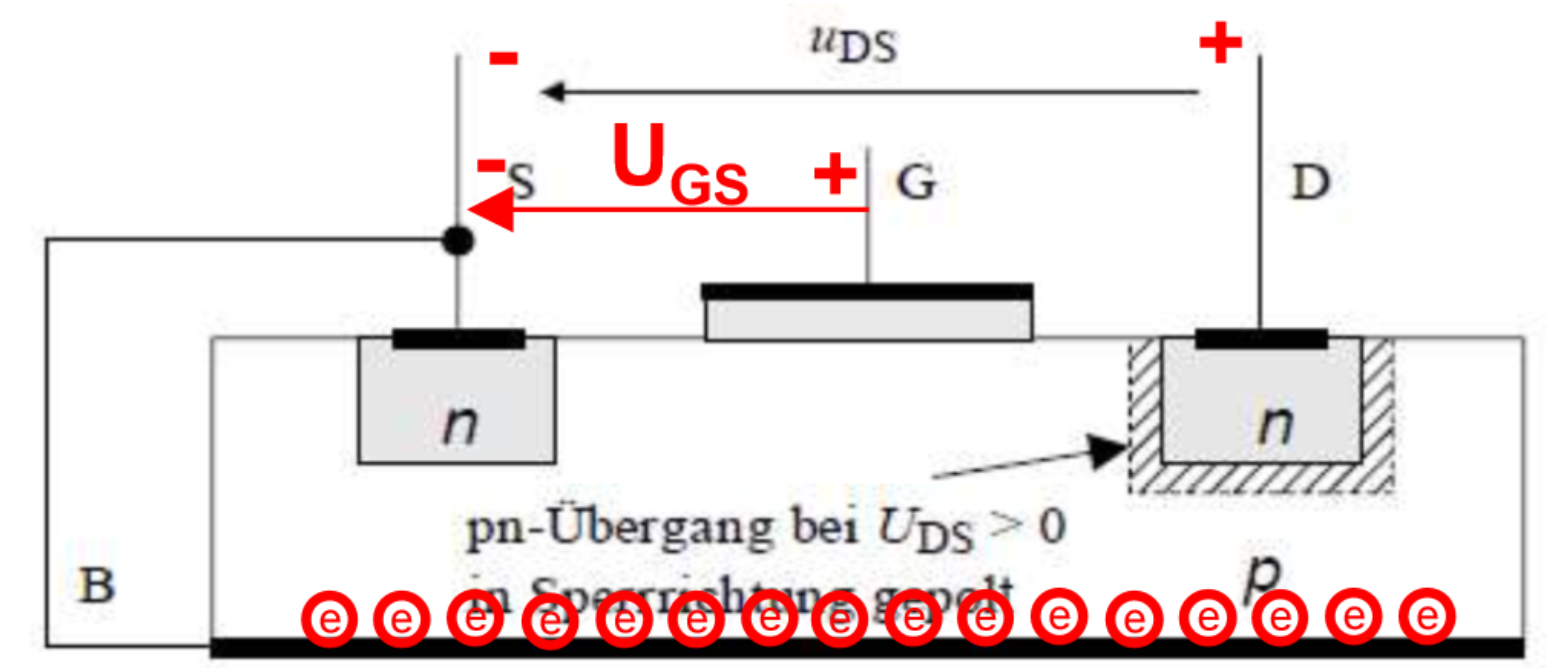
\includegraphics[width=\linewidth]{images/mosfetprak}
\end{wrapfigure}
Die elektrishe Leitfähigkeit des Substrats ist duch ein el. Feld gesteuert. Das el. Feld ruft im Substraht einee Influenzladung hervor.\newline
Die Gate-Elektrode ist durch ein Metaloxid vom Substraht isoliert.\newline
\vspace{0.4cm}
\begin{tabular}{ll}
    S = Source & D = Drain\\
    G = Gate & B = Bulk(Substraht)\\
\end{tabular}\newline
$ U_{DS} $ ist positiv damit ist der rechte pn-Übergang in Sperrrichtung gepolt. Deswegen kann keink Storm in beide Richtungen fliessen.\newline
$ \rightarrow $ Der Transistor ist selbstsperrend.\newline
\danger Sobald eine positive Spannung zwischen $ G $ und $ S $ angelegt ist, entsteht ein leitfähiger n-Kanal und damit auch ein Strom vom D- zum S-Anschluss.
 \vspace{-0.2cm}
\subsection{IGBT}
Der IGBT setzt such aus einem Bipolartransistor $ T_2 $ und einem MOSFET $ T_1 $ zusammen.\newline
    n- ist eine schwach dotierte Zone, welche zut Erhöhung der Spannungsfestigkeit verwendet wird.
\begin{center}
  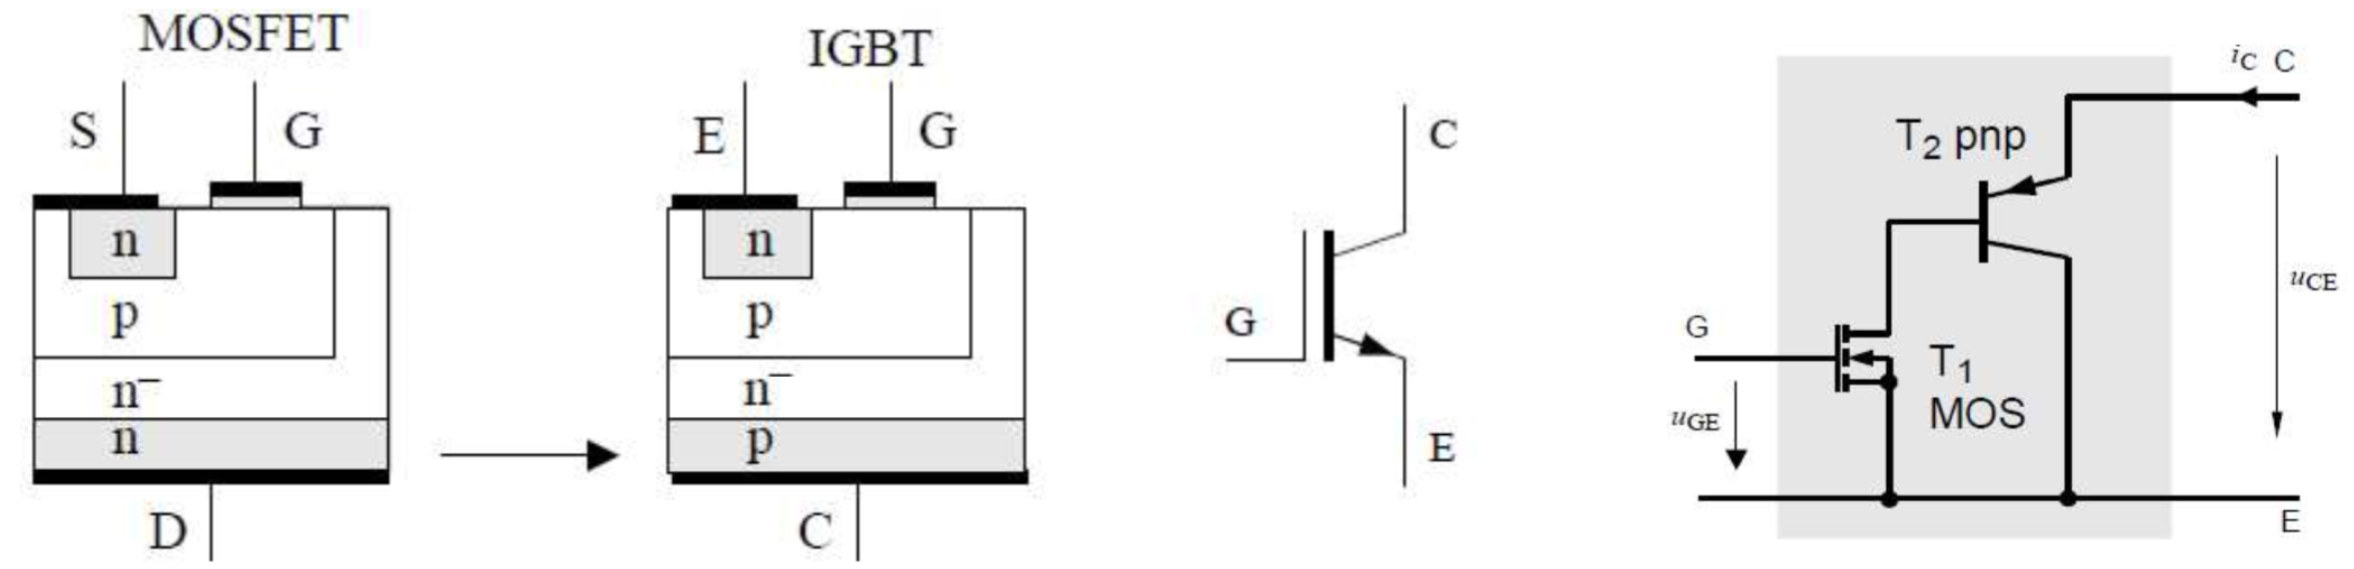
\includegraphics[width=0.7\linewidth]{images/IGBTaufbau}
  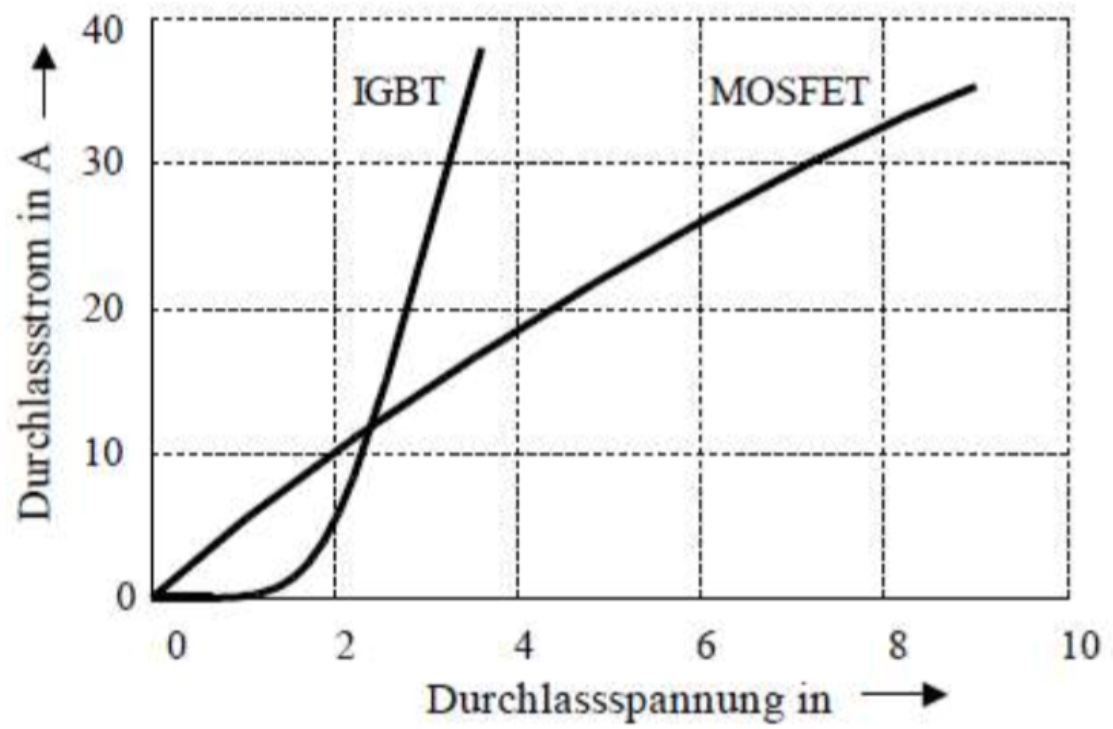
\includegraphics[width=0.25\linewidth]{images/IGBTkennlinie}
\end{center}
\vspace{-0.5cm}
\subsubsection{Eigenschaften}
\begin{multicols}{2}
    \begin{itemize}
        \item Über die Kollektor-Emitter-strecke fällt mindestens die Schleusenspannug ab
        \item kleine Durchlassverluste bei hehen Ströme
        \item in Rückwärtsrichtung nur begrenzt Sperrfähig
        \item Grosse Sperrverluste vorallem beim Abchlaten
    \end{itemize}
\end{multicols}
\clearpage

\subsection{Transistoren im Vergleich}
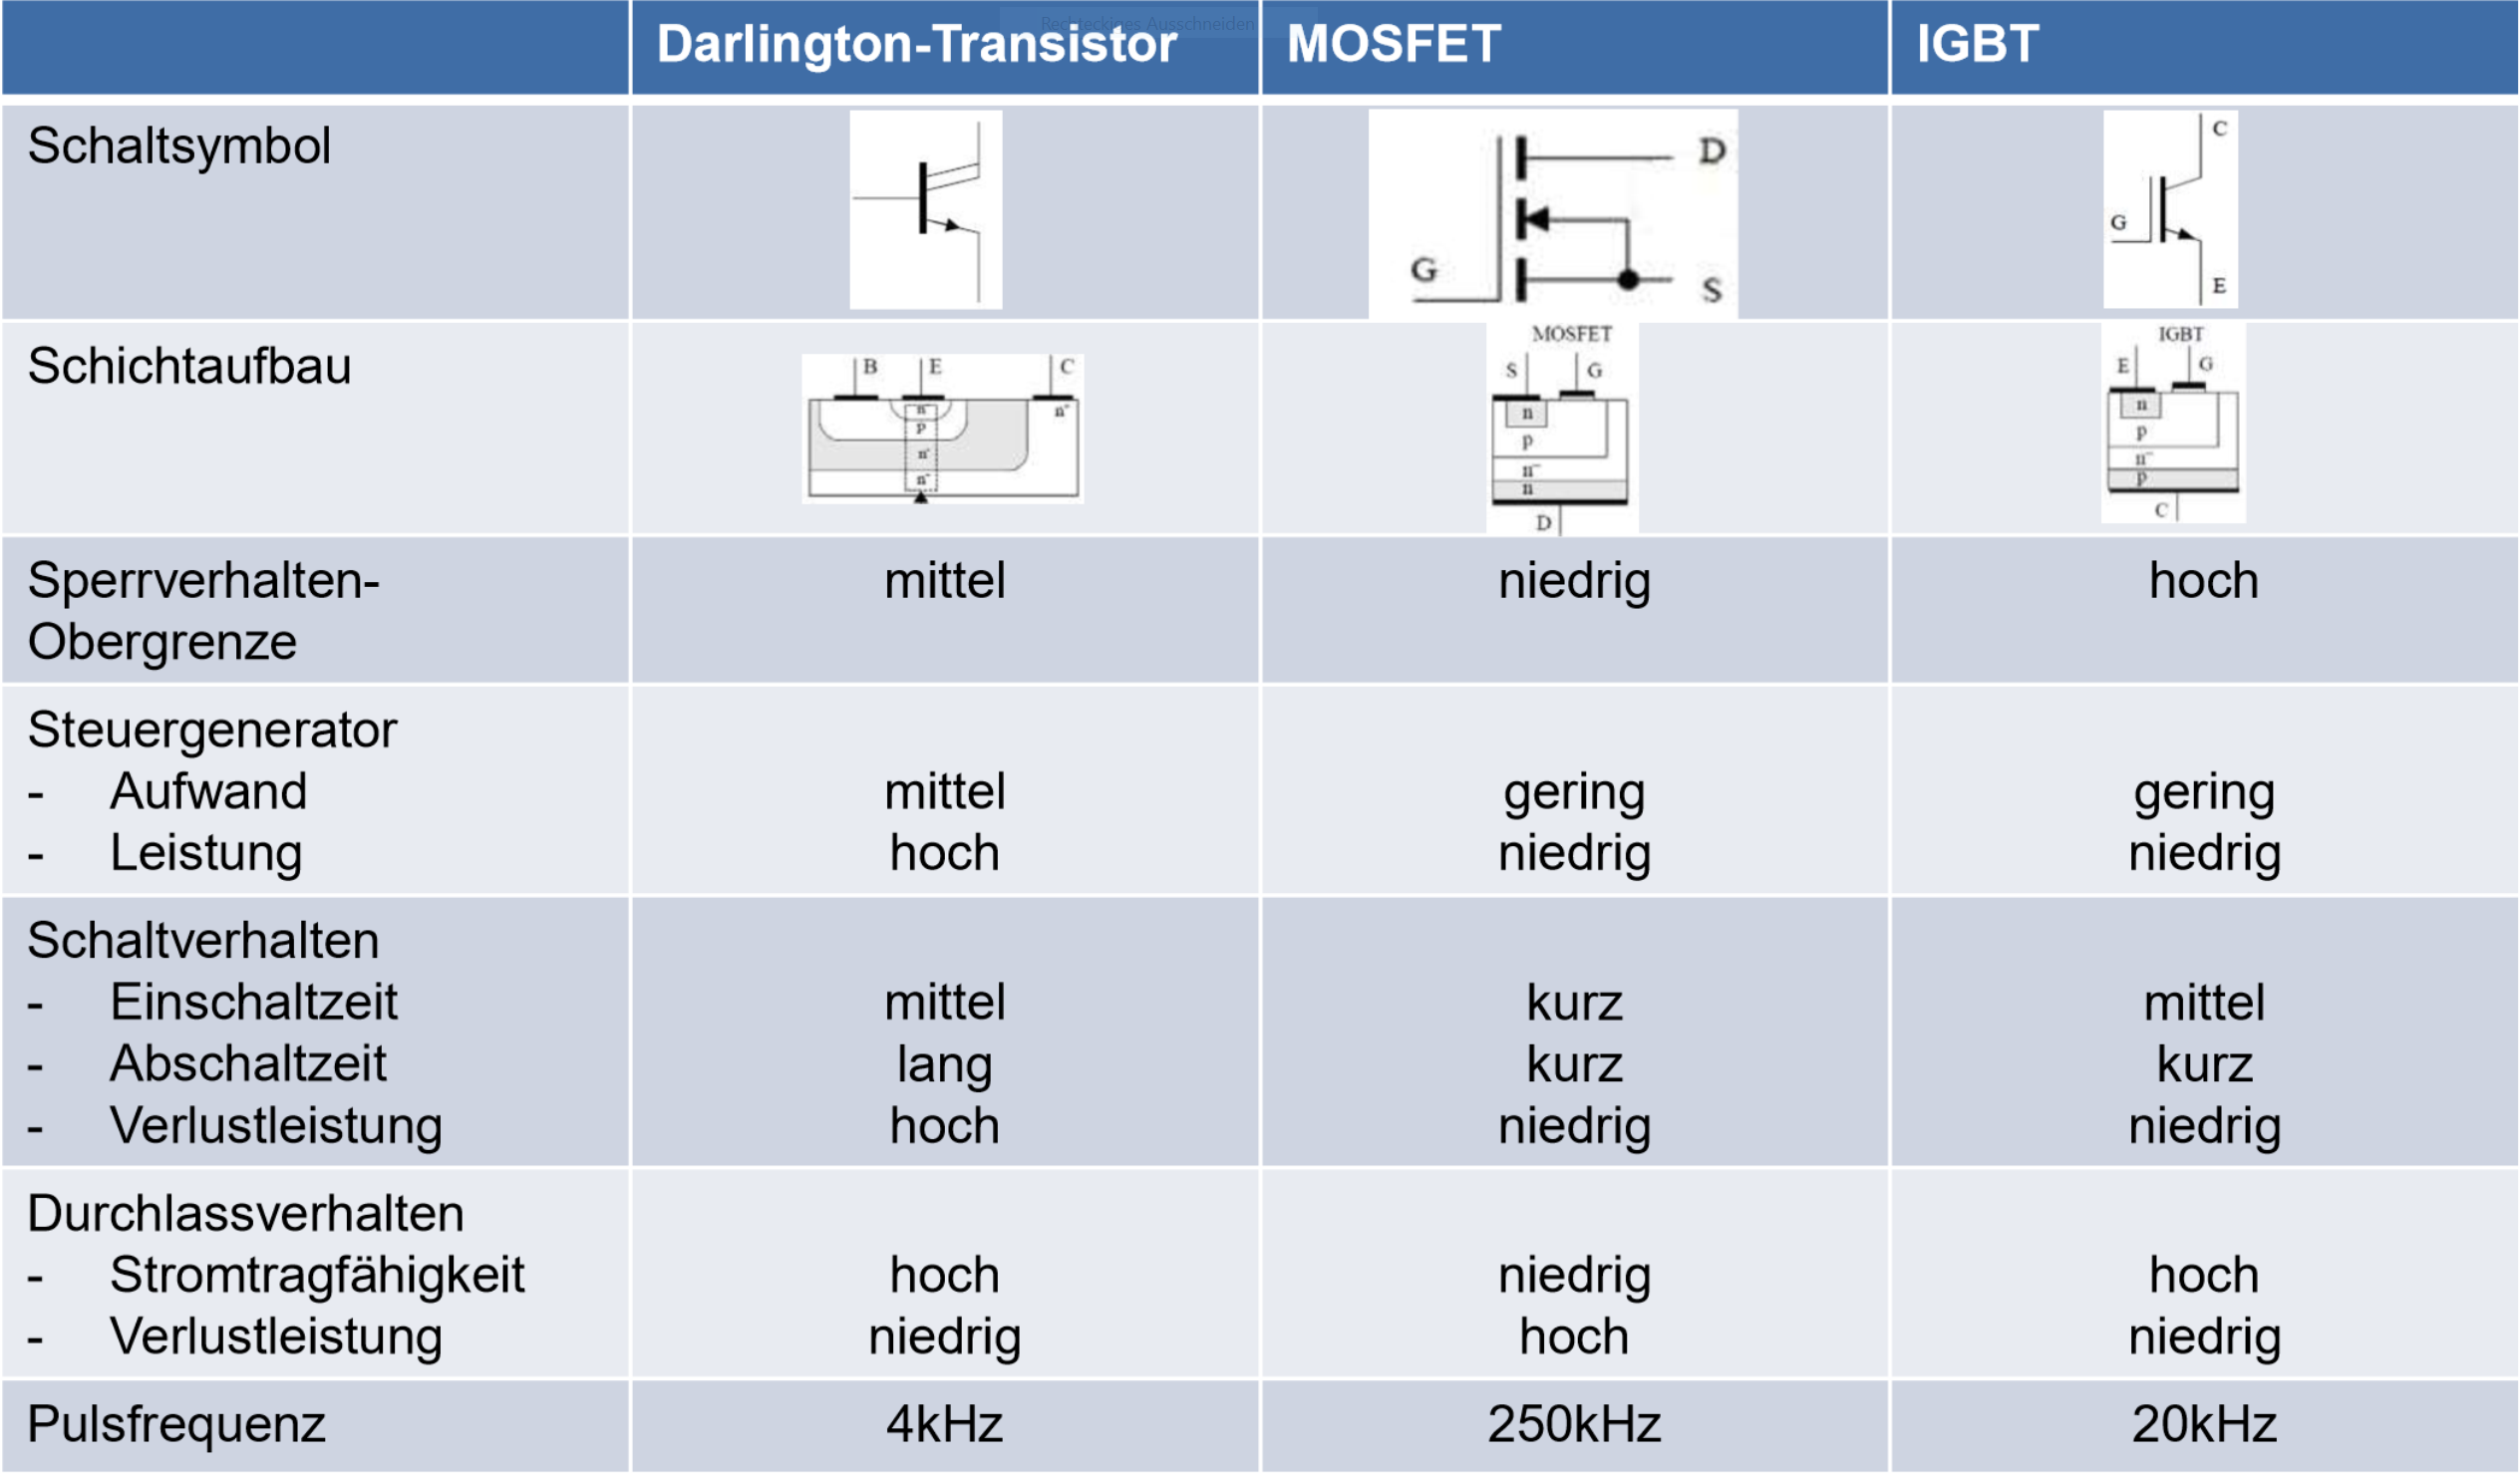
\includegraphics[width=\linewidth]{images/transdiff}
%\begin{tabular}{lccc}
%    &\textbf{Darlington-Transistor}&\textbf{MOSFET}&\textbf{IGBT}\\
%    Schaltsymbol&
%    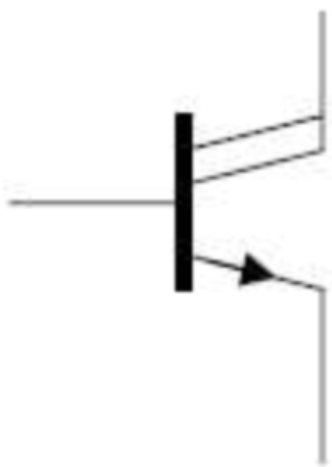
\includegraphics[width=1cm]{images/darlingtonSymbol}&
%    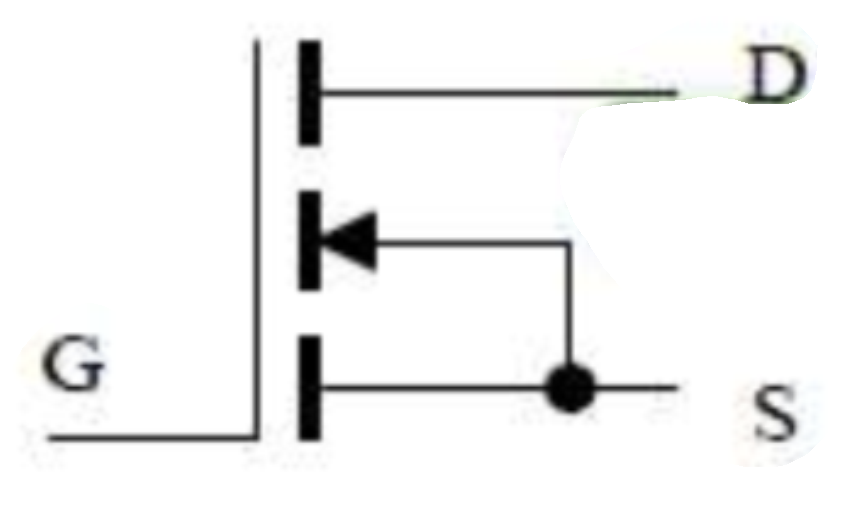
\includegraphics[width=2cm]{images/MOSFETSymbol}&
%    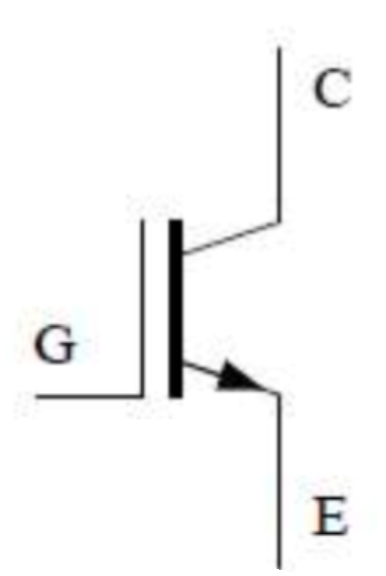
\includegraphics[width=1cm]{images/IGBTSymbol}\\
%    
%    Schichtaufbau&
%    \includegraphics[width=1cm]{images/darlingtonSchicht}&
%    \includegraphics[width=1cm]{images/MOSFETSchicht}&
%    \includegraphics[width=1cm]{images/IGBTSchicht}\\
%    
%    &&&\\
%    &&&\\
%    &&&\\
%    &&&\\
%    &&&\\
%    &&&\\    
%\end{tabular}

%=========================================
\clearpage